\PassOptionsToPackage{pdfpagelabels=false}{hyperref}

\documentclass[fleqn,usenatbib,useAMS]{mnras}

\setlength{\topmargin}{-0.3in}
\usepackage{graphicx}
\usepackage{amsmath}
\usepackage[dvipsnames]{xcolor}  
\usepackage{amssymb}
\usepackage{color}
\usepackage[figure,figure*,table,table*]{hypcap}

\hypersetup{draft}

\listfiles

\input{macros.sty}

\title[Satellite Kinematics -- Application to SDSS]
	{The galaxy--halo connection from satellite kinematics\\ -- II. Application to SDSS}
\author[J.~U.~Lange et al.]
{Johannes~U.~Lange$^1$\thanks{email: johannesulf.lange@yale.edu}, Frank~C.~van~den~Bosch$^1$ and Andrew~R.~Zentner$^2$\\
	$^1$Department of Astronomy, Yale University, P.O. Box 208101, New Haven, CT 06511, USA\\
	$^2$Department of Physics and Astronomy \& Pittsburgh Particle Physics, Astrophysics, and Cosmology Center (PITT PACC),\\University of Pittsburgh, Pittsburgh, PA 15260, USA}

%\date{Accepted XXX. Received YYY; in original form ZZZ}
\pubyear{2017}

\begin{document}

\date{Accepted xxx. Received xxx}

\label{firstpage}
\pagerange{\pageref{firstpage}--\pageref{lastpage}}

\maketitle

\begin{abstract}
	XXX
\end{abstract}

\begin{keywords}
methods: statistical -- galaxies: kinematics and dynamics -- galaxies: groups: 
general -- cosmology: dark matter
\end{keywords}

\section{Introduction}

\section{Observational Data}
\label{sec:data}

Observational constraints in this work come from the New York University Value-Added Galaxy Catalog \citep[VAGC;][]{Blanton+05}. This catalogue is derived from the Seventh Data Release of the Sloan Digital Sky Survey \citep[SDSS DR7;][]{Abazajian+09}. Specifically, we use the \texttt{bright0}\footnote{\url{http://sdss.physics.nyu.edu/lss/dr72/bright/0/}} of the VAGC. This includes roughly $\sim 570,000$ galaxies with a limiting Petrosian magnitude of $m_r < 17.6$. $k$-corrections and evolution corrections to redshift $z = 0.1$ have been applied to all galaxies in the sample. We then require an $r$-band luminosity of $L > 10^{9.5} \Lsunh$. We apply the same $g - r$ colour cut to divide galaxies into red and blue as used by \cite{Zehavi+11}. Note that this cut is slightly different than the cut \cite{More+11} applied. The colour cut can be written as
\begin{equation}
	(g - r)_{\rm cut}^{0.1} = 0.21 - 0.03 (M_r^{0.1} - 5 \log h).
\end{equation}
Due to mechanical limitations, spectroscopic fibres cannot be placed simultaneously for objects separated by less than $55''$ on the sky. Due to these fibre collisions around $\sim 6\%$ of the targets lack a spectroscopic redshift. In this case, we use the nearest-neighbour redshift assignment scheme \citep{Zehavi+05}. 

\subsection{Sample Selection}

As described in Paper I, we use a cylindrical isolation criterion to identify central candidates. A galaxy is considered isolated, a primary, if it does not have another brighter galaxy within a cylindrical volume defined by depth $(\Delta v)\rmh$ and radius $R_\rmh$. Any other fainter galaxy inside this cylinder is removed from the list of potential primaries. The cylinder dimensions, as described below, are a function of the luminosity and colour of the galaxy in question. Additionally, we require primaries to have a spectroscopic redshift, i.e. no fibre collision, and to lie in the redshift range $0.02 < z < 0.067$. Furthermore, we remove galaxies close to the angular survey edge. This is characterized by putting a ring around each galaxy corresponding to the angular size of $R_\rmh$ at that galaxy's redshift and demanding that not more than $20\%$ of it lies outside the survey area. Finally, primaries are required to lie in a survey region with at least $80\%$ spectroscopic completeness. Afterwards, satellite candidates, so called secondaries, lying inside a cylinder defined by $(\Delta v)_\rms$ and $R_\rms$ are associated to each primary. Contrary to \cite{vdBosch+04} and \cite{More+09b, More+09a, More+11}, primaries are not removed if they have no secondary.

We follow \cite{vdBosch+04} and make the cylinder sizes dependent on the galaxy properties. This typically increases completeness and purity of the resulting sample of central and satellite candidates. Specifically, we choose $(\Delta v)_\rmh = 1000 \sigma_{200} (L, C)$, $R_\rmh = 0.5 \sigma_{200} (L, C) h^{-1} \Mpc$, $(\Delta v)_\rms = 4000 \kms$ and $R_\rms = 0.15 \sigma_{200} (L, C) h^{-1} \Mpc$. Here, $\sigma_{200} = \sigma / 200 \kms$ is an estimate for the velocity dispersion of satellites as a function of primary luminosity $L$ and colour $C$. Because this estimate is a priori unknown, the cylinder sizes must be extracted from the data itself in an iterative fashion. We start with an estimate for $\sigma_{200} (L, C)$ and extract primaries and secondaries. An estimate for $\sigma_{200} (L, C)$ is extracted from the data by fitting the distribution of secondaries in the $\Delta v_z$--$L_{\rm pri}$ plane. Here, $\Delta v_z$ is the line-of-sight velocity difference of the secondary and its primary and $L_{\rm pri}$ the luminosity of the primary. The model is
\begin{equation}
	P(\Delta v_z, L_{\rm pri}) = \frac{f_{\rm int}}{2 z_\rms} + \frac{1 - f_{\rm int}}{\sqrt{2 \pi \sigma^2} \mathrm{erf}(z_\rmh / \sqrt{2} \sigma)} \exp \left[ - \frac{\Delta v_z^2}{2 \sigma^2} \right],
\end{equation}
where both the interloper fraction $f_{\rm int}$ and the velocity dispersion $\sigma$ are a function of the primary luminosity. Specifically, $f_{\rm int}$ is assumed to be a linear function of $\log L_{\rm pri}$ and
\begin{equation}
	\log \sigma / \kms = a + b (\log L_{\rm pri} - 10) + c (\log L_{\rm pri} - 10)^2,
\end{equation}
where $a$, $b$ and $c$ are constants. The best fit is found by maximizing the likelihood,
\begin{equation}
	\mathcal{L} \propto \prod\limits_{\mathrm{secondaries}} P(\Delta v_{z, i}, L_{\mathrm{pri}, i})^{w_{\mathrm{sw}, i}},
	\label{eq:likelihood_mem}
\end{equation}
where $w_{\mathrm{sw}, i}$ is a weight for each primary--secondary pair, as discussed in the next section. We then update our estimate for $\sigma_{200} (L, C)$ and extract a new set of primaries and secondaries. Using the best-fit values of \cite{More+11} as a a starting point, we find our algorithm to arrive at $a = 2.210$, $b = 0.478$, $c = 0.275$ and $a = 2.142$, $b = 0.402$, $c = -0.170$ for red and blue galaxies, respectively.

\begin{figure*}
	\centering
	\includegraphics{hist_sdss}
	\caption{The velocity distribution of secondaries in SDSS as a function of the luminosity of the associated primary. We split the secondaries by the colour of the primary, red (left panel) or blue (right panel).}
	\label{fig:hist}
\end{figure*}

Figure \ref{fig:hist} shows the line-of-sight velocity distribution of secondaries around primaries of a given luminosity. We show the distribution around red and blue primaries separately. From this Figure it is apparent that the velocity dispersion is a strong function of primary luminosity for red primaries and less so for blue ones. We will analysis this more quantitatively in the coming sections.

\subsection{Constraints}

We seek to constrain the galaxy--halo connection using a set of observables extracted from the above data set. In short, those constraints are the overall number density of galaxies, the red fraction of primaries, the number of same-halo secondaries around primaries and their velocity dispersion. All quantities are measured in $10$ bins in $\log L / \Lsunh$ from $9.5$ to $11.0$.

The number density of galaxies is estimate via
\begin{equation}
	n_{\rm gal} = \frac{\sum w_{\rms, i}}{\frac{\Omega_{\rm SDSS}}{3} (d_{\rm com}^3 (z = 0.067) - d_{\rm com}^3 (z = 0.02))},
\end{equation}
where the sum goes over all galaxies with a spectroscopic redshift and $\Omega_{\rm SDSS} = 2.273 \mathrm{sr}$ is the effective survey area of SDSS. Finally, $w_{\rms, i}$ is a weight designed to correct spectroscopic incompleteness, as discussed in Paper I. For each galaxy, we count the number of neighbouring targets within $55''$. We then assign a weight that is the inverse of the fraction of targets with the same number of neighbours that have been assigned a spectroscopic redshift. Similarly, the red fraction of primaries is defined by
\begin{equation}
	f_{\rm pri, r} = \frac{\sum\limits_{\rm red \ primaries}w_{\rms, i}}{\sum\limits_{\rm all \ primaries} w_{\rms, i}}.
\end{equation}
For the rest of the constraints, we need to take into account that not all secondaries are satellites of the same halo as the primary. This is particularly important when evaluating the velocity dispersion.

As discussed in detail in Paper I, we fit the $\Delta v_z$--$R_p$ distribution of secondaries in each bin of primaries with a flat interloper model $P_{\rm int} (\Delta v_z, R_p)$ and a model for same-halo satellites $P_{\rm sat} (\Delta v_z, R_p)$. The phase-space distribution of satellites in a halo of fixed mass is discussed in the appendix. Furthermore, we assume that the host halo masses of the satellites are drawn from a log-normal distribution with mean and spread as free parameters. We determine the fit that maximises the likelihood and assign a membership probability
\begin{equation}
	p_{\rm mem} (\Delta v_z, r_p) = \frac{P_{\rm sat} (\Delta v_z, r_p)}{P_{\rm sat} (\Delta v_z, r_p) + P_{\rm int} (\Delta v_z, r_p)}
\end{equation}
for each secondary. When determining the fit that maximizes the likelihood, we assign a weight to each primary--secondary pair,
\begin{equation}
	w_{\mathrm{sw}} = w_{\mathrm{s, pri}} w_{\mathrm{s, scd}},
\end{equation}
the product of the spectroscopic weight of the primary and the secondary. Except for the fibre collision correction, this assign equal weights to all secondaries. Thus, quantities derived from this weighting scheme are satellite-weighted. We then estimate the number of same-halo secondaries via
\begin{equation}
	n_\rms = \frac{\sum\limits_{\rm secondaries} p_{\mathrm{mem}, i} w_{\mathrm{sw}, i}}{\sum\limits_{\rm primaries} w_{\rms, i}},
\end{equation}
where $w_{\mathrm{sw}}$ is the product of the spectroscopic weight of each secondary and its according primary.

Similarly, an estimate for the satellite-weighted velocity dispersion is obtained via
\begin{equation}
	\sigma_{\rm sw}^2 = \frac{\sum\limits_{\rm secondaries} p_{\mathrm{mem}, i} w_{\mathrm{sw}, i} \Delta v_{z, i}^2}{\sum\limits_{\rm secondaries} p_{\mathrm{mem}, i} w_{\mathrm{sw}, i}}.
\label{eq:sigma_sw}
\end{equation}
Finally, we wish to estimate the average velocity dispersion when weighting each primary or host instead of each secondary. We do so by first assigning each secondary a weight of
\begin{equation}
	w_{\mathrm{hw}} = \frac{w_{\mathrm{s, pri}} w_{\mathrm{s, scd}}}{N_{\rm scd}},
\end{equation}
where $N_{\rm scd}$ is the number of secondaries hosted by each primary. $\sigma_{\rm hw}$ is then calculated in complete analogy to $\sigma_{\rm sw}$.

Ultimately, we have up to $80$ constraints, $n_{\rm gal}$, $f_{\rm pri, r}$, $n_{\rm s, r}$, $n_{\rm s, b}$, $\log \sigma_{\rm hw, r}$, $\log \sigma_{\rm hw, b}$, $\sigma_{\rm hw, r}^2 / \sigma_{\rm sw, r}^2$ and $\sigma_{\rm hw, b}^2 / \sigma_{\rm sw, b}^2$, each measured in $10$ bins of primary luminosity and $n_{\rm s}$, $\log \sigma_{\rm hw}$ and $\sigma_{\rm hw}^2 / \sigma_{\rm sw}^2$ for red and blue primaries separately. However, we only consider data points for which we estimate to have at least $10$ primaries with at least $1$ same-halo secondary and for which we can create an uncertainty estimate, as described in the next section. In Table \ref{tab:data} we show an overview of the data used in this study. Note that this requires an assumed radial profile to get membership probabilities. For this data we assumed that satellite follow an NFW profile that is half as concentrated as that of dark matter.

\begin{table*}
	\begin{tabular}{lccccccccccc}
		\hline
		Description & \multicolumn{10}{c}{Bins} & Total\\
		\hline\hline
		$\log L_{\rm pri, min}$ & $9.50$ & $9.65$ & $9.80$ & $9.95$ & $10.10$ & $10.25$ & $10.40$ & $10.55$ & $10.70$ & $10.85$ & $9.50$ \\
		$\log L_{\rm pri, max}$ & $9.65$ & $9.80$ & $9.95$ & $10.10$ & $10.25$ & $10.40$ & $10.55$ & $10.70$ & $10.85$ & $11.00$ & $11.00$ \\
		\hline
		Red Primaries & $2693$ & $3138$ & $3430$ & $3186$ & $2715$ & $1871$ & $1042$ & $408$ & $95$ & $11$ & $18589$ \\
		Associated Secondaries & $10$ & $62$ & $178$ & $410$ & $706$ & $1060$ & $1313$ & $1230$ & $734$ & $152$ & $5855$ \\
		Blue Primaries & $7160$ & $6029$ & $4888$ & $3548$ & $2317$ & $1351$ & $526$ & $126$ & $17$ & $0$ & $25962$ \\
		Associated Secondaries & $8$ & $59$ & $151$ & $179$ & $240$ & $267$ & $132$ & $63$ & $7$ & $0$ & $1106$ \\
		\hline
		$\log n_{\rm gal} [h^{3} \mathrm{Mpc}^{-3}]$ & $-2.405$ & $-2.458$ & $-2.526$ & $-2.641$ & $-2.806$ & $-3.038$ & $-3.381$ & $-3.882$ & $-4.549$ & $-5.565$ & $-1.803$ \\
		$f_{\rm pri, r}$ & $0.273$ & $0.342$ & $0.413$ & $0.474$ & $0.543$ & $0.586$ & $0.675$ & $0.776$ & $0.866$ & $1.000$ &  \\
		$n_{\rm s, r}$ & -- & $0.013$ & $0.041$ & $0.095$ & $0.223$ & $0.514$ & $1.259$ & $3.423$ & $8.324$ & -- &  \\
		$n_{\rm s, b}$ & -- & -- & $0.019$ & $0.038$ & $0.081$ & $0.167$ & $0.204$ & $0.439$ & -- & -- &  \\
		$\sigma_{\rm hw, r} [\kms]$ & -- & $150.6$ & $157.4$ & $152.3$ & $224.7$ & $227.7$ & $257.4$ & $389.1$ & $423.6$ & -- &  \\
		$\sigma_{\rm hw, b} [\kms]$ & -- & -- & $90.0$ & $158.7$ & $135.3$ & $172.3$ & $218.0$ & $188.7$ & -- & -- &  \\
		$\sigma_{\rm hw, r}^2 / \sigma_{\rm sw, r}^2$ & -- & -- & -- & -- & $0.861$ & $0.772$ & $0.725$ & $0.450$ & $0.559$ & -- &  \\
		$\sigma_{\rm hw, b}^2 / \sigma_{\rm sw, b}^2$ & -- & -- & -- & -- & -- & $0.687$ & $0.837$ & $0.728$ & -- & -- &  \\
		\hline
	\end{tabular}
	\caption{Overview of the data used in this analysis. We have defined $10$ bins in the luminosity of the primary $\log L_{\rm pri}$. The first two rows show the bin edges and the next four rows the number of primaries and secondaries. Finally, the last eight rows show the constraints derived from the data that we use to constrain the model. Constraints that could not be measured or for which no reliable uncertainties could be derived from mocks are omitted.}
	\label{tab:data}
\end{table*}

\section{Model for Constraints}
\label{sec:model}

Ideally, one would compute all constraints in mock catalogues and directly compare those results to SDSS. Unfortunately, this is prohibitively expensive for our current analysis. Instead, we will employ a novel approach where we use a large number of mock catalogues to find the best-fit model and an analytical approach to evaluate uncertainties. In the following, we will briefly summarize the analytical model. We refer the reader to Paper I to a more detailed discussion of this model and how it fares in comparison to mock catalogues.

The number density of galaxies in a luminosity range $[L_1, L_2]$ can be inferred from the CLF combined with the halo mass function via
\begin{equation}
n_{\rm gal}(L_1, L_2) = \int\limits_{L_1}^{L_2} \int\limits_0^\infty \Phi_{\rm tot}(L | M) n_\rmh (M) \mathrm{d}M \mathrm{d}L.
\end{equation}
Here, $\Phi_{\rm tot}(L | M)$ is the combined CLF of central and satellites for a halo of virial mass $M$. The halo mass function $n_\rmh (M)$ is computed directly from the SMDPL simulation output. See the appendix for a discussion of the CLF parametrization.

The number red fraction of primaries can be approximated as the red fraction of centrals,
\begin{equation}
f_{\rm pri, r} (L_1, L_2) \approx \frac{n_{\rm c, r} (L_1, L_2)}{n_{\rm c, r} (L_1, L_2) + n_{\rm c, b} (L_1, L_2)}.
\end{equation}
The number density of centrals, similarly $n_{\rm gal}$ above, is computed by integrating the central CLF over the halo mass function in SMDPL.

The expected number of secondaries around primaries can be very well described by the corresponding number of satellites around centrals,
\begin{equation}
n_\rms (L_1, L_2) \approx \frac{\int\limits_{L_1}^{L_2}\int\limits_0^\infty N_\rms (M) n_\rmh (M) \Phi_\rmc (L | M) f_{\rm ap} (L, M) \mathrm{d}M \mathrm{d}L}{n_\rmc (L_1, L_2)}.
\end{equation}
Here, $N_\rms (M)$ is the expected number of satellites for a halo of mass $M$ and $\Phi_\rmc$ is the central CLF. $f_{\rm ap} (L, M)$ describes the fraction of satellites in a halo of mass $M$ with a central of luminosity $L$ that are expected to lie inside the cylinder defined by $R_\rms$,
\begin{equation}
f_{\rm ap} (L, M) = \int\limits_0^\infty 4 \pi r^2 \bar{n}_{\rm sat} (r | M) (\zeta(r, R_\rms (L)) - \zeta(r, R_\rmc)) dr,
\label{eq:f_ap}
\end{equation}
where $\bar{n}_{\rm sat}$ is the normalized radial profile of satellites in a halo of mass $M$,
\begin{equation}
\int\limits_0^\infty 4 \pi r^2 \bar{n}_{\rm sat} (r | M) dr = 1,
\end{equation}
and
\begin{equation}
\zeta(r, r_\rms) = \begin{cases}
1 &\quad\text{if } r \leq r_\rms \\
1 - \sqrt{1 - r_\rms^2 / r^2} &\quad\text{otherwise.} \\ 
\end{cases}
\end{equation}
Note that we have excluded those satellites lying inside $R_\rmc = 60 \kpch$ to correct for fibre collisions.

In a similar fashion, the velocity dispersion is approximated as the expected velocity dispersion of satellites around all centrals in a given luminosity range,
\begin{align}
\sigma^2 &(L_1, L_2) \approx \nonumber\\
&\frac{\int\limits_{L_1}^{L_2}\int\limits_0^\infty w (L, M) \sigma^2_{\rm ap} (L, M) n_\rmh (M) \Phi_\rmc (L | M) \mathrm{d}M \mathrm{d}L}{\int\limits_{L_1}^{L_2}\int\limits_0^\infty w (L, M) n_\rmh (M) \Phi_\rmc (L | M) \mathrm{d}M \mathrm{d}L}.
\end{align}
$w (L, M)$ is a weight set to
\begin{equation}
w_{\rm sw} (L, M) = f_{\rm ap} (L, M) N_\rms (M)
\end{equation}
for the satellite-weighted velocity dispersion and
\begin{equation}
w_{\rm hw} (L, M) = 1 - \exp \left( - f_{\rm ap} (L, M) N_\rms (M) \right)
\end{equation}
for the host-weighted velocity dispersion. Finally, $\sigma^2_{\rm ap} (L, M)$ is the expected average velocity dispersion of all satellites living inside a halo of mass $M$ and being inside the cylinder defined by $R_\rms(L)$
\begin{align}
\sigma^2_{\rm ap} & (L, M) = \nonumber\\
&\frac{\int\limits_0^\infty r^2 \bar{n}_{\rm sat} (r | M) \sigma^2 (r | M) (\zeta(r, R_\rms (L)) - \zeta(r, R_\rmc)) dr}{\int\limits_0^\infty r^2 \bar{n}_{\rm sat} (r | M) (\zeta(r, R_\rms (L)) - \zeta(r, R_\rmc)) dr}.
\end{align}
The expected velocity dispersion $\sigma^2 (r | M)$ at any given radial distance $r$ and halo mass $M$ is computed from the spherical Jeans equation without anisotropy. The expected velocity dispersion also needs the radial profile of satellites $\bar{n}_{\rm sat}$ as an input. Throughout this work, we test three different choices for the radial profile. One assumes that the satellite distribution can be described by an NFW profile with the same scale radius as the dark matter in each halo. Another choice is that satellites follow an NFW profile with a scale radius that is twice as large as that of the dark matter. Finally, we consider satellites having a cored profile that very well fits the distribution of resolved subhaloes in SMDPL (see Paper I). We will call these three choices NFW, bNFW and Cored, respectively.

\section{Analysis Procedure}
\label{sec:analysis}

The goal of this work is to constrain the galaxy--halo connection parametrized by the model vector $\boldsymbol{\theta} = \{L_{0, \rm r}, M_{1, \rm r}, \gamma_{1, \rm r}, ...\}$ by our observational data $\boldsymbol{D} = \{n_{\rm gal}, f_{\rm pri, r}, ...\}$. To do this we assume a likelihood of the form
\begin{equation}
	\mathcal{L}(\boldsymbol{\theta} | \boldsymbol{D}) \propto \exp \left[ - \frac{(\boldsymbol{M}^\star (\boldsymbol{\theta}) - \boldsymbol{D})^t \boldsymbol{\Psi} (\boldsymbol{M}^\star (\boldsymbol{\theta}) - \boldsymbol{D})}{2} \right],
	\label{eq:likelihood}
\end{equation}
where $\Psi$ is the precision matrix, i.e. the inverse of the covariance matrix, and $\boldsymbol{M}^\star (\boldsymbol{\theta}) = \langle \boldsymbol{D} (\boldsymbol{\theta}) \rangle$ the model prediction for the data vector. Both the model prediction and the covariance matrix are derived from detailed SDSS-like mock catalogues. However, the following simplifications are made in order to make the likelihood evaluation computationally feasible.

In the previous section, we have introduced a simple analytic model $\boldsymbol{M} (\boldsymbol{\theta})$ for the full forward-modelling prediction $\boldsymbol{M}^\star (\boldsymbol{\theta})$. In Paper I, we have shown that this simple model is able to reproduce all qualitative features of the forward-modelling prediction. At the same time, small biases between that model and results from mock catalogues of the order of $\sim 1 \sigma$ exists. Thus, we calibrate the analytic model such that it reproduces the forward-modelling prediction for a given set of parameters $\boldsymbol{\theta}_0$. Specifically, we introduce a bias vector $\boldsymbol{B (\boldsymbol{\theta}_0)} = \boldsymbol{M}^\star (\boldsymbol{\theta}_0) - \boldsymbol{M} (\boldsymbol{\theta}_0)$. We then approximate the forward-modelling prediction for an arbitrary model $\boldsymbol{\theta}$ as
\begin{equation}
	\boldsymbol{M}^\star (\boldsymbol{\theta}) \approx \boldsymbol{M} (\boldsymbol{\theta}) + \boldsymbol{B (\boldsymbol{\theta}_0)}.
	\label{eq:model}
\end{equation}
An estimate $\boldsymbol{\hat{B} (\boldsymbol{\theta_n})}$ for the bias vector is obtained from $1000$ mock catalogues created from model $\boldsymbol{\theta}_0$. $\boldsymbol{M}^\star$ in this case is simply the average of the $1000$ data vectors.

As with the bias vector, we assume that the covariance matrix does not change significantly around any given set of parameters $\boldsymbol{\theta}_0$. An unbiased estimate for the covariance matrix is
\begin{equation}
	\boldsymbol{\hat{C}} = \frac{1}{N_S - 1} \sum_i^{N_S} (\boldsymbol{D}_i - \langle \boldsymbol{D} \rangle) (\boldsymbol{D}_i - \langle \boldsymbol{D} \rangle)^t,
\end{equation}
where $\boldsymbol{D}_i$ is the data vector of the $i$-th out of $N_S$ mock catalogues and $\langle D \rangle$ the average of all. Finally, an unbiased estimate for the precision matrix is
\begin{equation}
	\boldsymbol{\hat{\Psi}} = \frac{N_S - N_D - 2}{N_S - 1} \boldsymbol{\hat{C}}^{-1},
	\label{eq:precision}
\end{equation}
where $N_D$ is the number of data points, i.e. the dimensionality of $\boldsymbol{D}$ \citep{Taylor+13}. We note that we only use data points which can be measured in all $1000$ mock catalogues and $\sigma_{\rm hw} / \sigma_{\rm sw}$ only if $n_{\rm sat} > 0.1$ on average. The latter constraint is mainly due to the distributions of $\sigma_{\rm hw} / \sigma_{\rm sw}$ in the mocks being very non-Gaussian otherwise.

\begin{figure}
	\centering
	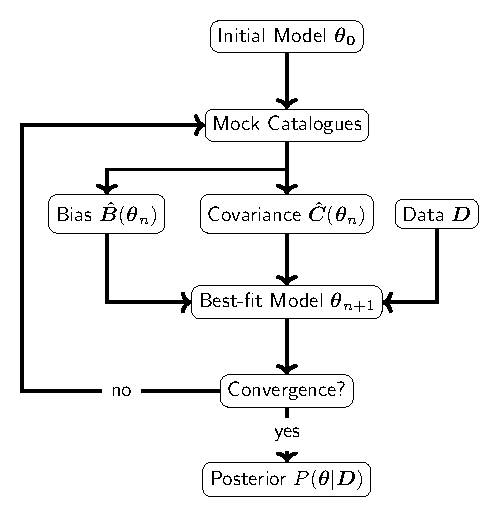
\includegraphics{graph}
	\caption{Diagram outlining our analysis procedure of the SDSS data. We start out with an initial model $\boldsymbol{\theta_0}$ and create mock catalogues. These mock catalogues are used to estimate the covariance of the data and the offset between the analytical model for the constraints and the forward-modelling results. Using these estimates, the analytical model and the actual SDSS data, a new best-fitting model $\boldsymbol{\theta_1}$ is obtained. This process is repeated until the sequence of best-fitting models $\boldsymbol{\theta}_{0, 1, ..., n}$ is reasonably converged. Afterwards, the full posterior is estimated using the analytical model and the bias and covariance from the latest mock catalogues.}
	\label{fig:graph}
\end{figure}

Figure \ref{fig:graph} outlines how we find that best-fitting model and corresponding uncertainties. We start out with an initial guess for the galaxy--halo connection given by $\boldsymbol{\theta_0}$. In this work, the initial guess is the default parameter set of Paper I. We then create mock catalogues for this particular choice of parameters and construct the bias vector $\boldsymbol{\hat{B}}$, precision and covariance matrix from them. These are then used to find a new best-fit model $\boldsymbol{\theta}_1$ using the simplified analytic model that maximizes the likelihood in equation (\ref{eq:likelihood}). From this model we create another series mock catalogues and re-compute the bias and covariance. Afterwards, a new best-fitting model $\boldsymbol{\theta_2}$ is found. This process is repeated until a convergence criterion is reached, signalling that the best-fit models do not change significantly. At this point the last bias and covariance estimates are used to compute the entire posterior using the analytic model.

\begin{figure}
	\centering
	\includegraphics[width=\columnwidth]{progress}
	\caption{Series of best-fitting models when fitting SDSS with the NFW satellite profile. We show the $\chi^2$ difference of each iteration with respect to the latest, $\boldsymbol{\theta}_3$. The model covariance and bias for this plot have been obtained from mocks constructed with $\boldsymbol{\theta}_2$. See the text for details.}
	\label{fig:convergence}
\end{figure}

How do we asses the convergence of this algorithm? We have a series of best-fit models $\boldsymbol{\theta}_{0,1,...,n}$ based upon different estimates for the bias and covariance. We now take the latest estimate for the latter and compute the $\chi^2$ of all $\boldsymbol{\theta}_{0,1,...,n}$. By construction, $\boldsymbol{\theta}_n$ will have the lowest $\chi^2$. On the other hand, previous iterations will have higher values because they used different estimates for the bias and covariance for the minimization. If the posterior of $\boldsymbol{\theta}$ were described by a multivariate Gaussian distribution with $16$ degrees of freedom, $68\%$ of all models would lie within $\Delta \chi^2 = 18$ of the best-fit model. Thus, if $\chi^2 \left(\boldsymbol{\theta}_{n - 1} \right) - \chi^2 \left( \boldsymbol{\theta}_n \right) < 18$, the best-fitting model did not change significantly from the previous iteration and we regard the result as converged. An example is shown in Figure \ref{fig:convergence} where we show the $\chi^2$ series when fitting a model with the NFW profile to the SDSS data. Convergence is achieved at the third iteration. The initial model $\boldsymbol{\theta_0}$ gives an insufficient fit to the data with $\Delta \chi^2 \sim \chi^2 \sim 10000$. Thus, we cannot expect estimates for the bias and covariance matrix estimated from such mock catalogues to be very realistic with respect to SDSS. Nevertheless, the new best-fitting model $\boldsymbol{\theta_1}$ estimated from these estimates is only $\Delta \chi^2 \sim 25$ \jul{(Might be updated later.)} from the final best-fit model $\boldsymbol{\theta_3}$ away. Finally, $\boldsymbol{\theta_2}$ found using the bias and covariance estimate from $\boldsymbol{\theta_1}$ has $\Delta \chi^2 \sim 4$ \jul{(Might be updated later.)} when compared to $\boldsymbol{\theta_3}$ which is constructed from the bias and covariance estimates from $\boldsymbol{\theta_2}$.

We note that the bias estimate $\boldsymbol{\hat{B}}(\boldsymbol{\theta})$ of the analytic model used to find $\boldsymbol{\theta_3}$ has been calibrated at $\boldsymbol{\theta}_2$. Specifically, that means that the expected constraints have been fully forward-modelled for $\boldsymbol{\theta}_2$. For our full posterior, only $\sim 1\%$ \jul{(Might be updated later.)} of all models have a $\chi^2$ as good or better than $\boldsymbol{\theta}_2$. Thus, a model very close to the best-fitting parameter has been verified with a large number of mock catalogues.

For finding the best-fitting model, as well as estimating the posterior, we make use of MultiNest \citep{Feroz+08, Feroz+09} and its \texttt{Python} implementation \texttt{PyMultiNest} \citep{Buchner+14}. In all cases, we use a set of $10,000$ live points and a stopping criterion of $\Delta \ln \mathcal{Z} = 10^{-4}$, where $\mathcal{Z}$ is the estimate for the global Bayesian evidence. In case of finding a best-fitting model, we run \texttt{MultiNest} in constant efficiency mode and a target efficiency of $50\%$. On the other hand, when estimating the posterior, we de-activate the constant efficiency mode and set a target efficiency of $1\%$. Although not its main purpose, \texttt{MultiNest} is an extremely robust global minimization scheme that does not get stuck in local minima. To verify that our estimate for the posterior is fully converged, we have re-run \texttt{MultiNest} with $50,000$ live points and a target efficiency of $0.5\%$ and getting consistent results. \jul{Again, I'll do it in the end. I firmly believe that this will be the result.}

\section{Results}

We have performed the analysis procedure described in the above section for the three different satellite radial profiles separately. In each case, we used the specific radial profile to determine likely interlopers, produce mock catalogues and fit the data. We find that the observational constraints we used so far cannot reliably distinguish between the different models, all giving very similar $\chi^2$. Thus, we first analyse the observed radial profile of secondaries around primaries to distinguish between the different possible radial profiles. Afterwards, we will explore the fit to the data for the best-fitting radial profile in more detail.

\subsection{Radial Profile}

\begin{figure*}
	\centering
	\includegraphics{profile_sdss}
	\caption{The projected number density of secondaries around primaries of different luminosities. Data points are from SDSS. The bands show the predictions of the best-fitting models for each assumed radial profile. For each best-fitting model, we create $1000$ mock catalogues and the bands denote the $68\%$ containment in each bin. Overall, the bNFW profile matches the SDSS data the best.}
	\label{fig:profile}
\end{figure*}

Figure \ref{fig:profile} shows the predictions for the projected number density of primaries around secondaries. Each panel shows the distribution for different primary luminosities without distinction by the colour of primaries. Blue crosses denote the SDSS data and bands the predictions from each of the three posteriors. The bands present the $68\%$ scatter from $1000$ mock catalogues. Since for each mock we picked a random model from the posterior, bands show the combination of posterior uncertainty and statistical fluctuations due to cosmic variance. For both the mocks and the SDSS data, we have reduced the impact of interlopers by only considering secondaries within $600 \sigma_{200}(L, C) \kms$. On the other hand, we have increased $R_\rms$ from $0.15 \sigma_{200} \Mpch$ to $0.5 \sigma_{200} \Mpch$ to increase the range that is probed. A correction for fibre collisions has been applied by weighing each primary and secondary by $w_{\mathrm{s, pri}}$ and $w_{\mathrm{sw}} = w_{\mathrm{s, pri}} w_{\mathrm{s, scd}}$, respectively.

As expected, more radially extended profiles also predict the most shallow surface number densities. For example, the Cored profile predicts the lowest surface density at low radii and the largest at large radii. Overall, the model bNFW where satellites follow an NFW profile with a scale radius twice that of dark matter seems to fit the SDSS data the best. Thus, in the following we will concentrate on empirical results on the galaxy--halo connection derived from this radial profile.

\subsection{Model for Satellite Kinematics}

\begin{figure*}
	\centering
	\includegraphics{constraints_sdss}
	\caption{Observational constraints from SDSS (data points) and the best-fitting model (line). We show the number density of galaxies (top, left), the red fraction of primaries (top, right), the estimated number of satellites around primaries (bottom, left), the host-weighted velocity dispersion (bottom, middle) and the ratio of host to satellite-weighted velocity dispersion (bottom, right). All observables in the bottom row are measured separately for red and blue primaries. We also show the $\chi^2$ for each set of observations separately in each panel. Error bars represent the diagonals of the covariance matrix estimated from mock catalogues. The best-fitting model assumed the bNFW satellite profile.}
	\label{fig:constraints}
\end{figure*}

In Figure \ref{fig:constraints} we show the measurement values previously reported in Table \ref{tab:data}, together with $1\sigma$ error bars derived from mock catalogues and the best-fitting model. Qualitatively, the model excellently reproduces most trends in the observational data. The only exception is the ratio of host to satellite-weighted velocity dispersion for low-luminosity blue primaries. We believe that this is a purely statistical outlier based on two reasons. First, we see in the mock catalogues that the data points for a fixed model are only approximately distributed as Gaussian. Thus, such a $3 \sigma$ outlier is not as unlikely as for a Gaussian distribution. Secondly, \cite{More+11} did not observe such a low ratio blue primaries in the same luminosity range. Thus, we regard the best-fit model as a qualitatively very good description of the SDSS data. However, expressed via the $\chi^2$, the best-fit model is not a good fit to the data with $\chi^2 = 84.9$ for $61 - 16$ degrees of freedom. Thus, given that the model reproduces all qualitative trends of the data, our observational constraints seem to suggest a more complicated model for the galaxy--halo connection then assumed thus far. We will return to this point later in this section.

\begin{figure*}
	\centering
	\includegraphics{vz_sdss}
	\caption{The velocity distribution of secondaries around primaries for SDSS (data points) and the best-fitting bNFW model (bands). Each panel represents a different primary luminosity. We show the results for red and blue primaries separately. Bands show the $68\%$ containment prediction from the best-fitting model for $1000$ mock catalogues. Note that the $y$-scale in each panel is logarithmic in the upper half and linear in the lower in order to show the full dynamic range of the data. Overall, the best-fitting model is able to reproduce all qualitative trends in the data.}
	\label{fig:vz}
\end{figure*}

In Figure \ref{fig:vz} we show the full velocity distribution of secondaries with respect to interlopers. We concentrate on six different bins in primary luminosity, differentiating between secondaries around red and blue primaries. Data points come from SDSS and bands denote the $68\%$ range from $1000$ mock catalogues derived from the best-fitting model. Again, error bars are purely indicative of cosmic variance fluctuations. We have mitigated the effect of fibre collisions by weighting each primary-secondary pair by $w_{\mathrm{sw}} = w_{\mathrm{s, pri}} w_{\mathrm{s, scd}}$. No correction for interlopers has been applied. We note that the model has only been fitted to reproduce the second moment of the velocity distribution of satellites. On the other hand, higher order moments and the contribution of interlopers are all implicit predictions. Reassuringly, the best-fit model seems to accurately predict all of those.

\subsection{Galaxy--Halo Connection}

\begin{figure*}
	\centering
	\includegraphics{posterior_compact_sdss}
	\caption{Marginalized posteriors for the galaxy--halo connection for the bNFW radial profile. We do not show parameters related to the satellite occupation, $\alpha_s$, $b_0$, $b_1$ and $b_2$, and the low-mass slopes of the mass-luminosity relation, $\gamma_{1, \rmr}$ and $\gamma_{1, \rmb}$, as they are poorly constrained. The diagonal shows marginalized 1D posteriors and off diagonal panels the 2D posteriors. In the latter case, lines demarcate the $68\%$, $95\%$ and $99\%$ containment of the posterior.}
	\label{fig:posterior}
\end{figure*}

\begin{table}
	\centering
	\begin{tabular}{c|c|c}
		\hline
		Parameter & Posterior & Best-fit \\
		\hline\hline
		$\log L_{\rm 0, r}$ & $9.877^{+0.062}_{-0.045}$ & $9.904$ \\
		$\log M_{\rm 1, r}$ & $11.06^{+0.23}_{-0.13}$ & $11.15$ \\
		$\gamma_{\rm 1, r}$ & $3.52^{+0.95}_{-1.20}$ & $3.01$ \\
		$\gamma_{\rm 2, r}$ & $0.232^{+0.011}_{-0.011}$ & $0.230$ \\
		$\sigma_{\rm r}$ & $0.1692^{+0.0055}_{-0.0056}$ & $0.1690$ \\
		$\log L_{\rm 0, b}$ & $10.238^{+0.070}_{-0.088}$ & $10.312$ \\
		$\log M_{\rm 1, b}$ & $11.42^{+0.14}_{-0.17}$ & $11.56$ \\
		$\gamma_{\rm 1, b}$ & $3.27^{+0.91}_{-0.55}$ & $2.73$ \\
		$\gamma_{\rm 2, b}$ & $0.082^{+0.055}_{-0.048}$ & $0.037$ \\
		$\sigma_{\rm b}$ & $0.1780^{+0.0075}_{-0.0081}$ & $0.1787$ \\
		$f_0$ & $0.3908^{+0.0095}_{-0.0097}$ & $0.3929$ \\
		$\alpha_f$ & $0.446^{+0.014}_{-0.013}$ & $0.444$ \\
		$b_0$ & $-0.460^{+0.027}_{-0.028}$ & $-0.460$ \\
		$b_1$ & $0.538^{+0.060}_{-0.058}$ & $0.537$ \\
		$b_2$ & $0.059^{+0.023}_{-0.024}$ & $0.061$ \\
		\hline
	\end{tabular}
	\caption{Posterior predictions and best-fit values of all parameters described the galaxy--halo connection. We assumed the bNFW satellite profile, i.e. that satellites follow an NFW profile with a scale radius twice as large dark matter scale radius.}
	\label{tab:posterior}
\end{table}

\begin{figure}
	\centering
	\includegraphics{model_post_sdss}
	\caption{The marginalized posteriors on the galaxy--halo connection. We show the mass-luminosity relation for red and blue centrals (upper, left), the scatter in central luminosity at fixed halo mass for red and blue centrals (upper, right), the red fraction of centrals as a function of halo mass (lower, left) and the average occupation with satellites above $10^{9.5} \Lsunh$ (lower, right). Bands denote $68\%$ and $95\%$ containment ranges of the posterior.}
	\label{fig:model_post}
\end{figure}

Figure \ref{fig:posterior} shows marginalized posteriors for a subset of the parameters describing the galaxy--halo connection. Most parameters are tightly constrained with only the low-mass slopes $\gamma_{1, \rmr}$ and $\gamma_{1, \rmb}$ and the low-luminosity slope of the satellite CLF $\alpha_s$ being strongly limited by the prior. We also see tight correlations between certain parameters, for example the characteristic luminosity $L_0$ and the characteristic mass $M_1$ of the mass-luminosity relation for red and blue centrals, in good agreement with \cite{Cacciato+13} and \cite{Zu+15}. We list all posterior predictions on the parameters in describing the galaxy-halo relation in Table \ref{tab:posterior}. We include the median and $1\sigma$ ranges as well as the best-fit value for each parameter. Figure \ref{fig:model_post} summarizes the multidimensional posterior by showing predictions for key statistics of the galaxy--halo relation. Specifically, we show the prediction for the mass-luminosity relation, the scatter in luminosity at fixed halo mass, the red fraction of centrals as a function of mass and the satellite occupation above $10^{9.5} \ \Lsunh$. Interestingly, we find mass-luminosity relations that are very similar for red and blue centrals. The same is true for the scatter in luminosity. We also find that the red fraction increases with halo mass and reaches unity by roughly $\log M_{\rm vir} / \Msunh \sim 13$. We note that the prediction for the red fraction of lower mass haloes, $\log M_{\rm vir} / \Msunh \sim 11$, is purely an extrapolation of our model and is not constrained by data as we do not expect those haloes to host any galaxy above $10^{9.5} \ \Lsunh$. Finally, we find that the average number of satellites above $10^{9.5} \ \Lsunh$ should roughly scale linearly with the halo virial mass. We will compare all those results with previous studies on a more quantitative level in the next section.

\subsection{Testing Model Extensions}

Here, we test possible extensions to the default parametrization of the galaxy--halo connection. Specifically, we look at models with additional parameters compared to the standard parametrization. Instead of repeating the entire procedure described in \S \ref{sec:analysis}, we take the estimate of the covariance and bias from the best-fit default model and use the analytical model to evaluate the more complex one. In all cases, we assume the bNFW radial profile for satellites.

To judge the performance of extended models we look at evidence ratio. Note that for nested models one can show that the evidence ratio obeys
\begin{equation}
\frac{\mathcal{Z}(\boldsymbol{D} | M_{n})}{\mathcal{Z}(\boldsymbol{D} | M_{n + 1})} = \frac{P(\theta^{n + 1} = 0 | \boldsymbol{D})}{P(\theta^{n + 1})},
\end{equation}
where $\mathcal{Z}$ denotes the evidence and $M_n$ is the nested model of $M_{n + 1}$. Specifically, $M_{n + 1}$ reduces to $M_n$ for $\theta^{n + 1}$, the additional parameter of the complex model, being $0$. This makes it clear that the evidence ratio can be judged directly from looking at the marginalized posterior probability $P(\theta^{n + 1} = 0 | \boldsymbol{D})$.

\subsubsection{Mass-Luminosity Relation}

So far, we have parametrized the mass-luminosity relation of red and blue centrals via a broken power-law relation. In $\log M$--$\log L$ space, this roughly describes a piecewise linear relation with a low and a high-mass slope. We now add to this a quadratic term in $\log M$--$\log L$ space. This can be written as
\begin{equation}
L_\rmc (M) = L_0 \frac{(M / M_1)^{\gamma_1}}{(1 + M / M_1)^{\gamma_1 - \gamma_2}} \left( \frac{M}{M_1} \right)^{\gamma_3 \log (M / M_1)}.
\end{equation}
For $\gamma_3 = 0$, this relation reduces to the previous parametrization with low-mass slope $\gamma_1$ and high-mass slope $\gamma_2$. Thus, we introduce $2$ new free parameters, $\gamma_{3, \rmr}$ and $\gamma_{3, \rmb}$, for red and blue centrals respectively. We use priors in the range $[-0.3, +0.3]$ for both. Applying this more general model to SDSS yields marginalized posteriors of $0.003_{-0.022}^{+0.022}$ and $-0.158_{-0.086}^{+0.111}$ for $\gamma_{3, \rmr}$ and $\gamma_{3, \rmb}$, respectively. Thus, the data is compatible with $\gamma_3 = 0$ in both cases, indicating that this additional model freedom is not favoured by the SDSS analysis.

\subsubsection{Red Fraction of Centrals}

So far, we have assumed that the red fraction of centrals $f_\rmr (M)$ increases linearly with $\log M$ of the dark matter halo. We now increase the model complexity by including a quadratic term, such that
\begin{equation}
f_\rmr (M) = f_0 + \alpha_f \log M_{12} + \beta_f (\log M_{12})^2,
\end{equation}
where $M_{12} = M_{\rm vir} / 10^{12} \ \Msunh$. Furthermore, we demand that the red fraction increases with halo mass. Thus, for $\beta_f < 0$ and $\log M_{12} > - \alpha_f / (2 \beta_f)$, we set $f_\rmr (M) = f_0 - \alpha_f^2 / (4 \beta_f)$. Conversely, for $\beta_f > 0$ and $\log M_{12} < - \alpha_f / (2 \beta_f)$, we fix $f_\rmr (M) = f_0 - \alpha_f^2 / (4 \beta_f)$. Thus, this more general model also allows for a red fraction that is constant above or below a certain halo mass. Evidently, for $\beta_f = 0$, this model reduces to the default parametrization. When choosing a prior of $[-0.5, 0.5]$, the posterior prediction is $-0.068_{-0.036}^{+0.072}$. We find that models where the red fraction does reach a non-unity value above a halo mass of $10^{13} \ \Msunh$ are slightly favoured by the data. However, the overall evidence ratio tells us that this model is not better in explaining the data than the default model.

\subsubsection{Satellite Occupation}

In principle, we might expect that at fixed halo mass the satellite occupation depends on the colour of the central galaxy. The reasoning for this is that galaxy colour might correlate with halo formation time, which in turn correlates with subhalo or satellite occupation. \jul{Frank, add your preferred citations here.} We test this by allowing the satellite CLF to vary depending on central colour, such that
\begin{equation}
\Phi_{\rm sat} (L | M , \mathrm{blue \ central}) = \zeta \times \Phi_{\rm sat} (L | M, \mathrm{red \ central}).
\end{equation}
We choose $[0.5, 2.0]$ as a prior for this boost factor $\zeta$ and find $0.80_{-0.12}^{+0.15}$ as the posterior probability. Thus, the posterior does not strongly exclude $\zeta = 1$ and the overall evidence ratio does not significantly favour this model over the default parametrization.

\section{Discussion}

One of the main goals of this work and Paper I is to improve the analysis of satellite kinematics compared to previous efforts. Specifically, we want to investigate previously reported tensions between results from satellite kinematics and other methods \citep[see e.g.][]{Leauthaud+12, Mandelbaum+16}. To this end, we compare our results obtained to those obtained from projected galaxy clustering \citep{Zehavi+11, Vakili+16, Zentner+16}, redshift space clustering \citep{Guo+15b}, group multiplicity functions \citep{Sinha+17} and combinations thereof. We note that such a juxtaposition is only superficial and a detailed comparison would involve analysing all those observables in our mock catalogues and compare them to SDSS. Nevertheless, it this effort should allow us uncover strong discrepancies, if present.

\subsection{Radial Profile of Satellites}

Our findings shown in Figure \ref{fig:profile} favour a radial distribution of satellites that is biased with respect to dark matter. While our results are consistent with satellites following an NFW profile, their concentration parameter is likely lower than that of dark matter in the same halo by a factor of around two. At the same time, the cored profile that fits the distribution of $M_{\rm peak}$ selected subhaloes, as described in Paper I, does not provide an adequate description of the SDSS data. Thus, satellites seem to follow a steeper profile than subhaloes. 

Many previous studies reported similar findings, particularly that satellite distributions follow an NFW profile \citep[see e.g.][]{vdBosch+05c, Yang+05, Guo+12a}. This is in contrast to the results of \cite{More+09b}, who argue that satellites follow a cored profile. As described in Paper I, this is likely due to \cite{More+09b} not correcting for fibre collisions in SDSS. The finding that satellites have a steeper radial profile than subhaloes but less centrally concentrated than dark matter is also in good agreement with independent studies \citep{Yang+05, Chen08} and hydrodynamical simulations \citep{Nagai+05, Vogelsberger+14}. Finally, we note for such comparisons, one should keep in mind that the exact radial profile of satellites will likely depend on the halo mass range and the properties of satellites due to colour and luminosity segregation \citep{Chen08, Guo+13}.

\subsection{Galaxy--Halo Occupation}

A detailed comparison with results from clustering and other methods is hampered by two complications. First, all observables like satellite kinematics or clustering will have a dependence on cosmology at fixed models for the galaxy--halo connection. Furthermore, there will be a dependence on the halo definition and the halo finder used. It is thus prudent to only compare results obtained under similar cosmological parameters and halo definitions. We compare our results to the studies of \cite{Guo+15b}, \cite{Zentner+16}, \cite{Vakili+16} and \cite{Sinha+17}. Coincidentally, all works assume cosmological parameters compatible with the recent results of \cite{Planck14}. Even more, all studies used halo catalogues derived with the \texttt{ROCKSTAR} halo finder \citep{Behroozi+13} and spherical over-density $M_{\rm vir}$ haloes. A second complication is that all those studies use colour-independent halo occupation distribution (HOD) models. Such models only describe the number of galaxies brighter than a luminosity threshold living in a halo of mass $M$. They do not inherently describe the entire luminosity distribution of galaxy, e.g. the mass-luminosity relation, or their dependence on the colour of the central galaxy. Thus, to allow a comparison we need to downgrade our CLF results to such an HOD framework.

\cite{Guo+15b} model the redshift space clustering of galaxies in SDSS using the framework of \cite{Zheng+16} to accurately and efficiently calculate correlation functions. Specifically, they model both the projected correlation function and the monopole, dipole and quadrupole moments of the redshift space clustering. Furthermore, in addition to HOD parameters, they fit parameters describing the central and satellite velocity bias. \cite{Zentner+16} and \cite{Vakili+16} use \texttt{halotools} \citep{Hearin+16} to fit the projected correlation function of galaxies in SDSS DR7. We note that the observational data used in \cite{Zentner+16} comes from \cite{Zehavi+11}, whereas \cite{Vakili+16} use data from \cite{Guo+15b}. Compared to \cite{Guo+15b}, they also specifically allow for the presence of galaxy assembly bias \citep{Zentner+14}. Finally, \cite{Sinha+17} also fit the friends-of-friends group multiplicity function in addition to the projected correlation function. Their focus lies on the realistic simulation of observational effects by comparing observational results to a large number of mock catalogues.

\begin{figure}
	\centering
	\includegraphics{bias_cen}
	\caption{Prediction on the average clustering bias of central galaxies above a given luminosity (upper panel). We compare predictions from \protect\cite{Guo+15b}, \protect\cite{Vakili+16}, \protect\cite{Sinha+17} and our results. All results include $68\%$ error bars. Predictions have been made assuming the \protect\cite{Tinker+08} halo mass function and \protect\cite{Tinker+10} model for the halo bias. We also directly compare the differences between this work and other studies at fixed luminosity (lower panel). The points are slightly offset in the horizontal direction to improve clarity. They all correspond to magnitude limits of $M_r^{0.1} = -19.0, -19.5, -20.0, -20.5, -21.0$ and $-21.5$.}
	\label{fig:bias_cen}
\end{figure}

To make a most ``fair'' comparison of our results with clustering studies, we analyse the average spatial bias of all centrals above a given luminosity threshold. This is most closely related to observables in galaxy clustering, specifically the clustering strength in the $2$-halo regime, and should test agreement with clustering predictions despite the different parametrizations of the galaxy--halo relationship. Due to the tight relation between halo mass and bias, it is also indicative of the average halo mass. In Figure \ref{fig:bias_cen} we show one such comparison between the results of this work (blue crosses) and those of \cite{Guo+15b} (red triangles), \cite{Zentner+16} (orange circles), \cite{Vakili+16} (grey squares) and \cite{Sinha+17} (turquoise triangles). In all cases, we made predictions by applying the HOD model to the \cite{Tinker+08} mass function and the bias description of \cite{Tinker+10}. Slight differences in the cosmological parameters and redshifts of the halo catalogues have been accounted for in the calculation of the halo mass function and the bias. For example, \cite{Sinha+17} use slightly different cosmological parameters and halo catalogues derived for redshifts $z = 0.054$ and $z = 0.132$ to model the $M_r^{0.1} = -19$ and $M_r^{0.1} = -21$ sample, respectively. On the other hand, \cite{Guo+15b}, \cite{Zentner+16} and \cite{Vakili+16} all use $z = 0$ catalogues. All results include $68\%$ posterior uncertainties. The predictions of \cite{Zentner+16} and \cite{Vakili+16} are from models without the possibility for assembly bias. The posterior from \cite{Sinha+17} is the one using the $\Mvir$ halo definition and without principal component analysis (PCA).

Overall, we see an excellent qualitative agreement between all studies compared here. In all works, the bias of central galaxies increases strongly with their luminosity. Given the tight correlation of halo mass with bias, this indicates a positive correlation between halo mass and galaxy luminosity. At larger luminosities, our results predict a slightly lower central galaxy bias than those of \cite{Guo+15b}, \cite{Vakili+16} and \cite{Sinha+17}. The disagreement is generally at the level of around $2 \sigma$. However, \cite{Zentner+16} predict values similar to our results. Note that, for example, for the $L > 10.5 \Lsunh$ ($M_r = -21.5$) sample, all clustering studies use a similar sample of galaxies with redshifts of up to $\sim 0.2$, whereas our results are derived with galaxies at lower redshifts. Thus, all other studies are intrinsically correlated at fixed luminosity and their findings cannot be regarded as independent. Thus, any apparent agreement should not be seen as evidence that true average spatial bias is indeed higher than inferred from our study.

In our work, we also constrain the scatter in luminosity at fixed halo mass. Unfortunately, this is not directly constrained by results of simple HOD fitting, so we cannot compare our results with the studies previously discussed. \jul{In principle, $\sigma_{\log M}$ in HOD models is related to the scatter in luminosity. However, these constraints are poor to begin with. So a comparison would not be useful. The comparison is also very difficult to make since it depends on the slope of the mass-luminosity relation and is not constrained in HOD models. Should I mention that here?} \cite{Yang+08} have estimated the scatter in luminosity as inferred from their group catalogues. To estimate group masses, they assumed a one-to-one relationship between total group luminosity of galaxies above $M_r^{0.1} < -19.5$ and halo mass. They find a scatter in BHG luminosity of around $\sigma \sim 0.15 \ \mathrm{dex}$ for red and blue BHGs, in good agreement with our result of $\sigma_r = 0.169_{-0.006}^{+0.006}$ and $\sigma_b = 0.178_{-0.008}^{+0.008}$. Only at the lower mass end, they find a scatter of $\sim 0.10 \ \mathrm{dex}$. However, for such low-mass groups, the central dominates the total group luminosity, and thereby the halo mass estimate. Thus, the inferred scatter is likely to be artificially suppressed. \cite{Cacciato+13} have analysed the luminosity function, galaxy--galaxy lensing and clustering in SDSS in order to constrain cosmological parameters. Nevertheless, the scatter in luminosity at fixed halo mass was a by-product of this analysis. They find $\sigma_c = 0.157_{-0.007}^{+0.007}$, without making a distinction between red and blue galaxies. It is straightforward to show that this scatter for all galaxies is related to the individual scatter of red and blue galaxies via
\begin{equation}
	\sigma_c^2 = f_r \sigma_r^2 + f_b \sigma_b^2 + 2 f_r f_b (\langle \log L_r \rangle - \langle \log L_b \rangle)^2,
\end{equation}
where $f_r$ and $f_b$ are the red and blue fraction of centrals at any given halo mass. As expected, the scatter is slightly increased if red and blue centrals have different average luminosities. For example, for $\sigma_r = \sigma_b = 0.17$, $f_r = f_b = 0.1$ and $|\langle \log L_r \rangle - \langle \log L_b \rangle | = 0.1$, we get $\sigma_c = 0.184$. Ultimately, bearing this in mind, our results imply a slightly larger scatter than what is found by \cite{Cacciato+13}, but still in reasonable agreement.

\begin{figure}
	\centering
	\includegraphics[width=\columnwidth]{fsat}
	\caption{Predictions on the satellite fraction of galaxies brighter than $10^{9.5} \Lsunh$ for various studies. Our results, as well as those of \protect\cite{Guo+15b}, \protect\cite{Vakili+16} and \protect\cite{Sinha+17}, have been derived assuming the \protect\cite{Tinker+08} halo mass function. Results for \protect\cite{Zehavi+11} are given directly in their respective studies. Error bars show the $1\sigma$ uncertainty.}
	\label{fig:fsat}
\end{figure}

In Figure \ref{fig:fsat} we compare predictions for the satellite fraction of galaxies above $L = 10^{9.504} \Lsunh$ ($M_r^{0.1} = -19$). We used the \cite{Tinker+08} mass function and accounted for slightly different cosmologies and redshifts to calculate the values for our work and those of \cite{Guo+15b}, \cite{Zentner+16}, \cite{Vakili+16} and \cite{Sinha+17}. We also include the results reported in \cite{Zehavi+11}, which are, however, derived under significantly different cosmological parameters. In this comparison, we note a stronger disagreement between different predictions than in the previous one. The results of \cite{Guo+15b} imply a satellite fraction of around $\sim 21 \pm 1 \%$, whereas our finding is $\sim 28 \pm 1 \%$. The results of \cite{Vakili+16} fall in between those two values, but with roughly three times larger uncertainties. \cite{Sinha+17} find a satellite fraction that is in good agreement with our findings and incompatible with those of \cite{Guo+15b}. \cite{Zentner+16} predict a similarly high fraction $\sim 32 \pm 4 \%$ but with the largest uncertainty. Finally, \cite{Zehavi+11} find $\sim 33 \pm 1 \%$, but for a different cosmology and halo definition. It is unclear at this point what the reason for the disagreement between the different studies is. Given that \cite{Zentner+16} and \cite{Vakili+16} only used the projected correlation function and find the satellite fraction to be loosely constrained, it seems that this observation is compatible with a large range of satellite fractions. On the other hand, taken at face value, the redshift space clustering \cite{Guo+15b} seems to imply a lower fraction than the group multiplicity function \cite{Sinha+17} and satellite kinematics.

\begin{figure}
	\centering
	\includegraphics[width=\columnwidth]{nsat}
	\caption{Posterior predictions on the satellite occupation above $10^{9.504} \Lsunh$ ($M_r^{0.1} = -19$) from several studies. Bands denote the $68\%$ posterior uncertainty. We compare the results of our work, \protect\cite{Guo+15b}, \protect\cite{Vakili+16} and \protect\cite{Sinha+17}.}
	\label{fig:nsat}
\end{figure}

We further explore this point in Figure \ref{fig:nsat}, where we show the satellite occupation as a function of halo mass. The threshold is $10^{9.504} \Lsunh$ ($M_r^{0.1} = -19$) in all cases. Qualitatively, the results all agree very well with each other. However, at lower masses, $\log \Mvir / (\Msunh) \sim 12 - 13$, the results of \cite{Guo+15b} imply a lower satellite occupation than our findings and those of \cite{Zentner+16} and \cite{Sinha+17}. On the other hand, at the high mass end, $\log \Mvir / (\Msunh) \gtrsim 14.5$, we find a higher satellite occupation than all other studies.

Altogether, we find a satisfactory agreement of our results with a variety of different studies. In all the comparisons here, we do not find our predictions to be strong outliers. Although certain tensions, especially for the satellite fraction, exist, they affect all studies together, not just the results of satellite kinematics. If there were truly a discrepancy in those results and satellite kinematics, it could be due to a variety of reasons. In addition to systematic uncertainties affecting satellite kinematics, which we will discuss in the next section, there are also uncertainties affecting the modelling of clustering and group multiplicity functions. A prime factor could be assembly bias, the fact that the spatial clustering of dark matter haloes depends on secondary halo properties other than halo mass \citep{Gao+05, Wechsler+06}. If the galaxy occupation is correlated with those secondary properties at fixed halo mass, it will affect the clustering at fixed values for the galaxy occupation as a function of halo mass \citep[see e.g.][]{Zentner+14, Hearin+16}. Another uncertainty is the radial profile of satellites. For example, all other studies assumed that satellites follow the dark matter radial profile in an unbiased fashion. Our results, on the other hand, imply that satellite are anti-biased with respect to dark matter. Another uncertainty is whether satellite numbers follow a Poisson distribution. Since clustering is a 2-point statistic, it is very sensitive to the second moment of the distribution. Furthermore, \cite{Guo+15b}, \cite{Vakili+16} and \cite{Sinha+17} all assumed the $5$-parameter model of \cite{Zheng+07} to model observational data. However, as argued by \cite{Sinha+17}, this model might not be flexible enough to fit a variety of observations. Finally, we note that the agreement between satellite kinematics and clustering likely depends on the cosmological parameters, as it does for clustering and lensing \citep{Cacciato+09, Cacciato+13}. Thus, we might expect an agreement between all those studies only under the right cosmological parameters.

\subsection{Caveats}

It is important to consider that several simplified assumptions have been made in this work that might potentially bias our inferences. A prime concern is that we have assumed that satellite galaxies obey the spherically symmetric, time-independent Jeans equation without anisotropy. However, it is known that satellite distributions are not generally spherically symmetric, do have some radial anisotropy \citep{Diemand+04, Wojtak+13} and are not fully relaxed, i.e. time-independent \citep{Ye+17}. Observationally, \cite{Guo+15a, Guo+15b} argue that satellite galaxies have a lower velocity dispersion than dark matter particles, if both follow the same radial distribution. Thus, both populations cannot simultaneously obey the Jeans equation in the form we assumed. Additionally, it is also well known that the halo core and the central galaxy are unlikely to be at rest with the entire halo \citep{vdBosch+05a, Behroozi+13, Guo+15a, Guo+15b, Guo+16, Ye+17}, something we have implicitly assumed.

\begin{figure*}
	\centering
	\includegraphics[width=\textwidth]{sdss_shps}
	\caption{Difference between the predicted kinematic observables when satellites are placed on subhaloes, as opposed to following the simplified analytical prescription. In all panels, we show the difference of the subhalo based mocks with respect to the analytical phase-space results. In each panel, the different colours denote the colour of the primary and the points are slightly offset horizontally for clarity. Error bars show the $68\%$ scatter between different mock realizations, as inferred from the analytical mocks.}
	\label{fig:shps}
\end{figure*}

In Paper I, we have addressed such concerns by analysing mocks were satellites are placed on subhaloes and centrals in the dark matter halo core. Evidently, all the simplifications are violated in such mock catalogues. Nevertheless, our inferences were not strongly biased with respect to the input parameters, indicating that those simplifications do not have a strong impact on observables. We perform a similar exercise here. We take the best-fit parameters of the Cored profile and create $100$ mocks were satellites are placed on subhaloes and centrals in the dark matter halo core. We then calculate the average of all observables and compare it to the case where satellites follow our analytic prescription. As we show in Figure \ref{fig:shps}, differences between the two predictions are generally below the $1\sigma$ level, especially for $\log \sigma_{\rm hw}$ and $\sigma_{\rm hw}^2 / \sigma_{\rm sw}^2$, for all luminosities and independent of whether the primaries are red or blue. Thus, if satellites would follow $M_{\rm peak}$-selected subhaloes, our simplifications would only have a mild impact on observables. Note however that such subhaloes have a different radial profiles than satellites in SDSS. Thus, these results might not be indicative of how well our simplifications fare with respect to satellites in SDSS. Finally, we note that for future work on satellite kinematics, one could use phase-space coordinates extracted from hydrodynamical simulations to model satellite populations.

Another potential concern is the fact that we do not have $100\%$ completeness in BHGs. Particularly, our selection criterion will be biased against low-luminosity BHGs in high-density regions. If the mass-luminosity relation had a dependence on environment, a scenario we do not model, then, similar to the effects of assembly bias in clustering, our inferences would be biased.

We also assumed that centrals are always BHGs in their respective halo. However, we know that this is not the case \citep{Skibba+11, Hikage+13, Wang+14, Hoshino+15, Lange+18a}. However, \cite{Lange+18a} have shown that this simplification only has a very small effect on the measured velocity dispersion. Nevertheless, generally this should lead our analysis to slightly overestimate halo masses.

\section{Conclusion}

\section*{Acknowledgements}

This research was supported in part by the National Science Foundation under Grant No. NSF PHY-1125915. FvdB and JUL are supported by the US National Science Foundation through grant AST 1516962. ARZ is funded by the Pittsburgh Particle physics Astrophysics and Cosmology Center (Pitt PACC) at the University of Pittsburgh and by the NSF through grant NSF AST 1517563. This work was supported by the HPC facilities operated by, and the staff of, the Yale Center for Research Computing.

This work made use of the following software packages: \texttt{matplotlib} \citep{Hunter07}, \texttt{SciPy}, \texttt{NumPy} \citep{vdWalt+11}, \texttt{Astropy} \citep{Astropy13}, \texttt{Cython} \citep{Behnel+11}, \texttt{halotools} \citep{Hearin+16}, \texttt{Corner} \citep{Foreman-Mackey+16}, \texttt{MultiNest} \citep{Feroz+08,Feroz+09, Feroz+13}, \texttt{PyMultiNest} \citep{Buchner+14}, \texttt{mangle} \citep{Hamilton+04, Swanson+08} and \texttt{pymangle}\footnote{\url{https://github.com/esheldon/pymangle}}. We also thank the open-source developers behind \texttt{Ubuntu}, \texttt{GNOME}, \texttt{Xfce}, \texttt{Spyder}, \texttt{JabRef}, \texttt{TexStudio} and \texttt{Terminator}. All the above mentioned software packages helped to greatly expedite this work.

We thank Hong Guo, Manodeep Sinha and Mohammadjavad Vakili for making the posteriors of their analysis available to us.

% https://www.cosmosim.org/cms/simulations/multidark-bolshoi-project/
The authors gratefully acknowledge the Gauss Centre for Supercomputing e.V. (www.gauss-centre.eu) and the Partnership for Advanced Supercomputing in Europe (PRACE, www.prace-ri.eu) for funding the MultiDark simulation project by providing computing time on the GCS Supercomputer SuperMUC at Leibniz Supercomputing Centre (LRZ, www.lrz.de).The Bolshoi simulations have been performed within the Bolshoi project of the University of California High-Performance AstroComputing Center (UC-HiPACC) and were run at the NASA Ames Research Center.

\label{lastpage}

\bibliographystyle{mnras}
\bibliography{bibliography}

\section*{Appendix A: Galaxy--Halo Connection}
\label{sec:galaxy_halo_connection}

Here, we briefly describe our parametrization of the galaxy--halo connection. We refer the reader to Paper I for a more in-depth discussion.

The occupation of dark matter halos with galaxies is governed by a CLF model. Particularly, the CLF specifies the average number of galaxies with a luminosity in the range $[L - dL/2, L + dL/2]$ residing in a halo of mass $M$. We split the galaxy occupation into a central and satellite component,
\begin{equation}
\Phi_{\rm tot}(L | M) = \Phi_\rmc (L | M) + \Phi_\rms (L | M).
\end{equation}

For the central galaxies, we choose two different parametrizations for red and blue centrals,
\begin{equation}
\Phi_\rmc (L | M) = f_\rmr (M) \Phi_{\rm c, r}(L | M)+ f_\rmb (M) \Phi_{\rm c, b}(L | M).
\end{equation}
Here, $f_\rmr (M) = 1 - f_\rmb (M)$ is the probability that a galaxy residing in a halo of mass $M$ is red. This probability is parametrized by
\begin{equation}
f_\rmr (M) = f_0 + \alpha_f \log M_{12},
\label{eq:colour_cen}
\end{equation}
where $M_{12} = M / [10^{12} \Msunh]$. We assume that every halo hosts exactly one central whose luminosity is drawn from a log-normal distribution with scatter $\sigma$,
\begin{equation}
\Phi_\rmc (L | M) dL = \frac{\log e}{\sqrt{2\pi \sigma_\rmc^2}} \exp \left[ \frac{(\log L - \log L_\rmc (M))^2}{2 \sigma_\rmc^2} \right] \frac{dL}{L}.
\end{equation}
The median luminosity, which can be different for red and blue centrals, is parametrized by
\begin{equation}
L_\rmc (M) = L_0 \frac{(M / M_1)^{\gamma_1}}{(1 + M / M_1)^{\gamma_1 - \gamma_2}}.
\end{equation}
Additionally, the scatter in central luminosity is allowed to be different for red and blue centrals. Altogether, $L_{0, \rmr}$, $M_{1, rmr}$, $\gamma_{1, \rmr}$, $\gamma_{2, \rmr}$, $\sigma_\rmr$, $L_{0, \rmb}$, $M_{1, rmb}$, $\gamma_{1, \rmb}$, $\gamma_{2, \rmb}$, $\sigma_\rmb$, $f_0$ and $\alpha_f$ are the free parameters governing the occupation of dark matter haloes with central galaxies.

The occupation of satellite galaxies is assumed to follow of Poisson distribution with expectation value
\begin{equation}
N_\rms (M) = \int\limits_{L_{\rm th}}^\infty \Phi_\rms (L | M) dL,
\end{equation}
where $L_{\rm th}$ is a luminosity threshold above which we populate dark matter haloes. Following \cite{Yang+08}, the CLF of satellite galaxies follows a modified Schechter function,
\begin{equation}
\Phi_\rms (L | M) = \phi_\rms^* (M) \left( \frac{L}{L_\rms^*(M)} \right)^{\alpha_\rms} \exp \left[ - \left( \frac{L}{L_\rms^* (M)} \right)^2 \right] \frac{dL}{L}.
\end{equation}
$\alpha_\rms$, a free parameter, describes the low-luminosity slope of the satellite CLF. $L_\rms^* (M)$ describes the position of the exponential cut-off. \cite{Yang+08} found that this is closely related to the average luminosity of centrals, $L_\rms^* (M) \sim 0.562 L_\rmc (M)$. Thus, we choose
\begin{equation}
L_\rms^*(M) = 0.562 L_{\rmc, \rmr} (M).
\end{equation}
We note that, in principle, this CLF model allows satellites to be brighter than centrals. We explicitly remove satellites that are brighter than their respective centrals from out mock galaxy catalogues. Finally, the overall mass-dependent normalization of the satellite CLF is described by
\begin{equation}
\log \left[ \phi_\rms^* (M) \right] = b_0 + b_1 \log M_{12} + b_2 (\log M_{12})^2.
\end{equation}
Finally, satellites are also randomly assigned colours based on the parametrization in eq. (\ref{eq:colour_cen}) with $f_{0, \rm sat} = 0.44$ and $\alpha_{f, \rm sat} = 0.14$ \citep[compare][]{Yang+08}. This colour assignment only matters in the rare cases that satellites are identified as primary candidates. Thus, we have $\alpha_\rms$, $b_0$, $b_1$ and $b_2$ as free parameters for the satellite CLF. 

Central galaxies are assumed to be located at the centre of each dark matter halo and to be at rest with the bulk halo velocity. On the other hand, satellite galaxies are assumed to follow spherically symmetric profile whose number density can be described by a generalized NFW profile,
\begin{equation}
n_\rms (r) \propto \left( \frac{r}{\mathcal{R} r_\rms} \right)^{-\gamma} \left( 1 + \frac{r}{\mathcal{R} r_\rms} \right)^{\gamma - 3},
\end{equation}
where $r_\rms$ is the scale radius of the dark matter profile. $\gamma$ and $\mathcal{R}$ are free parameters. For $\gamma = \mathcal{R} = 1$, satellites follow the dark matter distribution in an unbiased fashion and become increasingly shallow for smaller $\gamma$ and larger $\mathcal{R}$. In this work, we consider three choices for $(\gamma, \mathcal{R})$ to describe the SDSS data: $(1, 1)$ which we call ``NFW'', $(1, 2)$ referred to as ``bNFW'' and $(0, 2.5)$ which we call ``Cored''.
We assume that satellite galaxies obey the spherically symmetric Jeans equation without velocity anisotropy. In this case, the velocity dispersion at any given radius can be computed via
\begin{align}
\sigma^2 (r | \Vvir, c_{\rm vir}) =& \frac{c_{\rm vir} \Vvir^2}{\mathcal{R}^2 g(c_{\rm vir})} \left( \frac{r}{\mathcal{R} r_\rms} \right)^\gamma\left( 1 + \frac{r}{\mathcal{R} r_\rms} \right)^{3 - \gamma} \nonumber\\
&\int\limits_{r / r_\rms}^{\infty} \frac{g(y)\mathrm{d}y}{(y / \mathcal{R})^{\gamma + 2} (1 + y / \mathcal{R})^{3 - \gamma}},
\label{eq:Jeans}
\end{align}
where $\Vvir = G \Mvir / \rvir$ is the virial velocity and $c_{\rm vir} = \rvir / r_\rms$ the virial concentration. Finally,
\begin{equation}
g(y) = \ln (1 + y) - \frac{y}{1 + y}.
\end{equation}
Higher order moments of the velocity distribution are ignored because we also do not analyse them in this work.

\section*{Appendix B: Mock Catalogues}
\label{sec:mock_catalogues}

A key advantage of our study over works using satellite kinematics is to use detailed mock catalogues to estimate observables and their associated errors. Here, we outline how mock catalogues are created.

All mock catalogues used in this work are based on the SMDPL dark matter-only simulation. Specifically, we use the $z = 0$ ROCKSTAR \citep{Behroozi+13} halo catalogue\footnote{\url{http://yun.ucsc.edu/sims/SMDPL/hlists/index.html}}. From this, we extract all main haloes with a virial mass of $\Mvir \geq 3 \times 10^{10} \Msunh$, corresponding to $300$ times the dark matter particle mass in SMDPL. The cosmology used in SMDPL is the same as the one we assume. Furthermore, the halo mass resolution is more than sufficient to resolve galaxies above $10^{9.5} \Lsunh$ \citep[compare e.g.][]{Guo+15b, Sinha+17} and the volume of SMDPL is more than $10$ times bigger than the volume of SDSS we analyse. Thus, SMDPL is the ideal simulation to base our analysis on.

We use \texttt{halotools} to populate the dark matter catalogue with galaxies according to the CLF recipe described above. Specifically, for each dark matter halo, we first draw a colour for the central and afterwards a luminosity. For the satellites, we first calculate the expected occupation and then draw a number from a Poisson distribution with the same mean. Afterwards, we assign luminosities and colours based on the CLF parameters. Satellites that are brighter than their respective centrals are removed. Generally, this only eliminates roughly $1\%$ of the satellite population. For both the centrals and satellites we consider all galaxies above a luminosity of $10^9 \Lsunh$. This threshold is lower than that of galaxies we analyse in SDSS and is chosen to have a sufficient number of targets for potential fibre collisions. Finally, central galaxies are assigned the phase-space position of the halo core and satellites phase-space positions relative to that based on the assumed radial profile and the spherical Jeans equation.

Now having a real-space galaxy catalogue, we place a virtual observer with a random position and orientation inside the simulation box. We periodically repeat the galaxy catalogue to include all galaxies within $z = 0.15$. Next, we calculate apparent magnitudes for all galaxies, taking into account average $k$ and evolution corrections. We remove all targets with $m_r^{0.1} > 17.6$. Afterwards, redshift space distortions and SDSS spectroscopic redshift errors are simulated by perturbing the cosmological redshift $z$ of all galaxies by
\begin{equation}
\Delta z = (1 + z) \times \frac{(v_{\rm los} + \mathcal{N}(0, (35 \kms)^2))}{c},
\end{equation}
where $v_{\rm los}$ is the line-of-sight velocity and $\mathcal{N}(0, (35 \kms)^2)$ represents a random variable drawn from a Gaussian distribution with $0$ mean and $35 \kms$ dispersion. Afterwards, we apply the NYU VAGC \texttt{bright0} survey window and mask. Finally, we simulate fibre collisions. For each galaxy in the catalogue, we determine all other targets within an angular separation of $55''$. We make a table of all galaxies having such close neighbours. We then remove a random galaxy from that list. Furthermore, with a probability of $65\%$ we assign all close neighbours still on the list the redshift of this galaxy and also remove them. This process is repeated until all galaxies have been removed from the table. In Paper I, we have shown that this fibre collision scheme, although simplified compared to what happens in SDSS \citep{Blanton+03}, is sufficient for our mock catalogues.

\end{document}
